\documentclass[12pt]{article}

\usepackage[a4paper, total={7in, 9in}]{geometry}
\usepackage{graphicx}
\graphicspath{ {./images/} }
\usepackage{xcolor}
\usepackage{algorithm}
\usepackage{algorithmic}
\usepackage{hyperref}
\usepackage{tabularx}
\usepackage{listings}


\setlength{\footskip}{50pt}

\begin{document}
\begin{titlepage}
	\title{RFIDNetwork User Manual}
	\author{Ben S. Duggan\\Indiana University: School of Informatics, Computing and Engenering\\dugganbens@gmail.com}
	\date{Last edit: \today\\
	Pre-release v0.9.0}
\end{titlepage}

\maketitle
\tableofcontents
\pagebreak

\section{Preface}
RFID technology has become cheaper and more accessible making it possible for a large number of readers to be deployed.  While this delivers a large amount of useful data it can be hard to collect and manage it.  For this reason this system was designed which collects reads from RFID readers and wirelessly transmits them to a central server.  The goal of the system was to make an open-source system to wireless collect, store and manage RFID data.\\\\
To implement the system each reader needs to have an Arduino and radio module.  However, if the reader is Arduino based, like the ETAG, then only a radio module is needed.  To save the read to the server you simply need to pass the RFID tag into the RFIDNetwork class and it will be wireless sent to the server.  It is up to the person running the code to get the RFID tag onto the Arduino and into the RIFDNetwork class (as this is largely reader specific) but sample code for the ETAG is provided along with code to use get reads from readers with RS-232 serial port, like the Gen. 2 reader.\\\\
The server is a Raspberry Pi (RPi) microcomputer and the Zero W is recommended as it is low cost, low power and comes with a Wifi module, but any RPi should work.  Additionally the server needs a real time clock (RTC) to know what time it is and a radio module to communicate with the Arduinos.  The RPi stores all of the RFID reads it received and runs a web server that allows users to view or manage the RFID data.\\\\
All of the code and documentation is stored on GitHub at \href{https://github.com/BenSDuggan/RFID-Network/}{github.com/BenSDuggan/RFID-Network/}.  If you find a problem with the code you can email me at dugganbens@gmail.com or create and issue on the GitHub page.\\

\section{Instillation}
This section shows how to install the system.  While I have tried to make the system easy to install, there are some things which cannot be avoided like soldering.  Most of the things that you will find difficult are things lots of people have had to learn on their own (including me) so you shouldn't be disgruntled.  If you get stuck with something you can probably find the answer with a quick Google search.  Most things are explained thoroughly but the one thing I can't help with is teaching you to solder.  Soldering is the technique to electrically connect two wires.  If you haven't soldered before just watch this video \url{https://www.youtube.com/watch?v=BLfXXRfRIzY} (or any other you can find) and  practice on some spare wires.  You can pick up a cheap soldering iron on amazon for less than \$30.\\
With that said if you have any problems you can send me an email and I'll try to help.  I've also made a video showing the entire installation process.  You can find it here: \url{}. \colorbox{pink}{make video}\\

\subsection{The radio}
For this system to work every device in the network needs to communicate with each other.  This is done using the nRF24L01+PA+LNA Wireless Transceiver or shortened to the nRF24.  This is a 2.4-2.48 GHz transceiver which means that it can send and receive data at the same frequency your WiFi uses.  Each radio has the option of using 126 different channels (different field sites) different transmission speeds (250 KBPS, 1 MBPS and 2 MBPS) and 4 different power settings.  It can connect to 6 other radios (expanded to 127 in software) and has a \textless 1 mA sleep power consumption.  You can find out more about the radios by viewing the datasheet (\url{https://www.sparkfun.com/datasheets/Components/SMD/nRF24L01Pluss_Preliminary_Product_Specification_v1_0.pdf}).\\
There are two common versions of the nRF24: short range and long range (see long range below).  From my testing the short range version are inadequate under almost all circumstances so only the long range should be used.  The long range model has an advertised range of 1000 m but I have only tested up to 600 m (more on the radio tests in section 6.1).  To allow for greater range and more than 6 radios to be connected a software library is used which creates a mesh network.  This is explained in section 4.3.  These radios and the RFIDNetwork class rely on the SPI protocol, so while it has only been tested on Arduinos and Raspberry Pis it should work on other microcontrollers that support SPI. You can also find everything needed with approximate pricing in the appendix (7.1)\\
The radio comes with 8 2.54 mm pins called male headers.  The recommended way to connect the radio is by soldering male headers to the microcontroller and then connecting a wire with female headers between the microcontroller and radio.  See the image below.  A modification needs to be made to the radios to ensure reliable performance due to an inadequate supply of power to the IC of the radio.  This can be done by buying a power module (seen in the image below) or soldering a 4.7$\mu$F-10$\mu$F capacitor between the ground and VCC pin (1 and 2) on the radio module.\\
\begin{center}
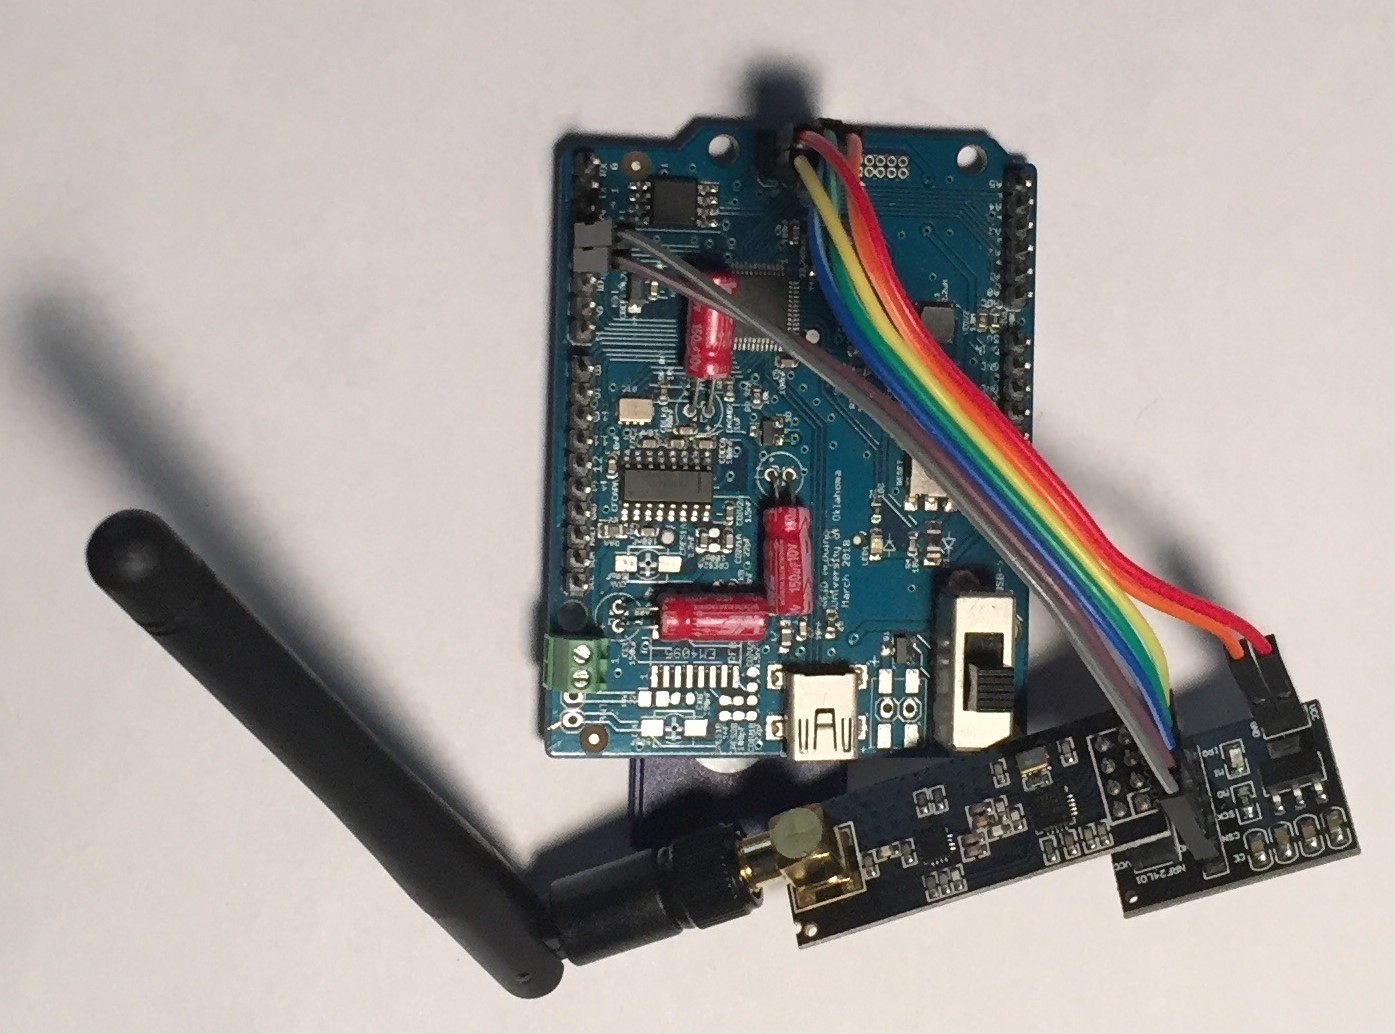
\includegraphics[width=6in,angle=180]{ETAG_Assembled}\\
ETAG with headers soldered on and female jumper wire connecting long range nRF24 with power module to board.
\end{center}
\subsubsection{Setting up the radio}
The radio will come in a static protector bag.  Take it out of the bag and screw the antenna onto the receptacle.  It should look like the image above.  To ensure reliable performance either a power module or capacitor needs to be added.  The power module makes it easier to switch in the field but is more expensive and uses more power (due to having a power indicator LED)than the capacitor.  The capacitor requires soldering but is cheaper and should result in the same performance.\\\\
\textbf{Using the power module:}
Notice that there are two rows of 4 male pins on the radio and 2 rows of 4 female pins on the power module.  Insert the radio into the power module so that all pins are seated.  Next connect 7 female wires to the wires on the power module.  Make sure that every pin on the power module is connected except for the pin labeled IRQ (looks like RO).  Make sure that you only plug the \textbf{VCC (pin 2) into 5V} otherwise the module might get enough power.  This should look like the picture above.\\\\
\textbf{Using the capacitors:}
It is recommended to use a 4.7-10 capacitor with the radio.  Solder the capacitor between pins 1 and 2 of the top of the radio (pin 1 has the white square around it and 2 is the the right, in the different row of 4 pins).  If you're using an electrolytic capacitor then make sure the negative lead is soldered to VCC.  Next connect 7 female wires to the wires on the radio.  You don't need to attached the IRQ (pin 8, located farthest away from pin 1 and on the side closer to the antenna).  Make sure that you plug the \textbf{VCC (pin 2) into 3.3V} otherwise the module might get damaged.  This should look like the picture below:
\begin{center}
	\colorbox{pink}{long range with capacitor and wires}
	%\includegraphics[width=6in]{nRF24_radioCap}\\
	Long range nRF24 radio with capacitor and wires attached.
\end{center}
\begin{center}
	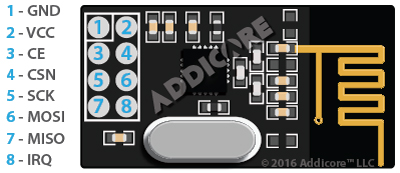
\includegraphics[width=6in]{nRF24_pinout}\\
	nRF24 pin layout with numbering and purpose.
\end{center}

\subsection{Arduino (RFID reader)}
The Arduino is used to get the RFID tag onto the server and saved.  This system should work with any RFID reader but you need to get the reads onto an Arduino supported microcontroller.  With Arduino based readers, like the ETAG, there is no need to purchase another Arduino as it is open-source and Arduino based.  However, with other readers that aren't Arduino based, like the Gen. 2 by Eli Bridge et al., a device must be used to get the reads onto an Arduino.  This makes the setup more complicated and more expensive.  We'll use both of these RFID readers as examples of how this system can be setup.  The software ran on the Arduinos is the same regardless of the reader, just will a few minor changes.
\subsubsection{Hardware}
\underline{\textbf{Arduino based RFID readers (e.g. ETAG)}}\\\\
To connect the radio to the Arduino (either an Arduino based RFID reader or one that will be used to communicate with a reader) you just need to connect the jumper wires from the radio to the board.  This means identifying which pins are used for SPI, digital, ground and power pins are (making sure you correctly use either 3.3V or 5V, depending on your configuration).
The easiest way to identify where the SPI pins are is by using the 6 pin ISCP header.  You may need to solder pins to it but it has as standard format (shown below).  The VCC is likely at 5V so if you are using the capacitor you \textbf{shouldn't use this VCC} and should use the 3.3V output pin and the board.  The ISCP VCC pin on the ETAG is at 5V.\\
\begin{center}
	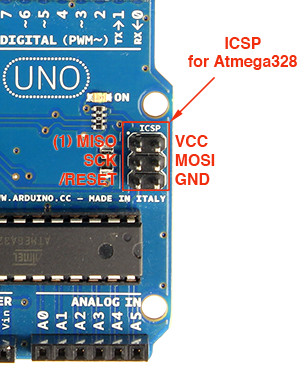
\includegraphics[width=6in,height=3in,keepaspectratio]{icsp_pinout}\\
	ISCP 6 pin header on Arudino Uno(ETAG) with pins labeled.
\end{center}
That takes care of GND, VCC, SCK, MOSI, MISO and IRQ (which isn't used).  The CE and CSN pin need to be connected to two digital pins and is defined in software.  By default CE is set to digital pin 3 and CSN is set to digital pin 4 but you can change this if you'd like.  This boils down to the following wiring as shown in the table below and the image showing the final setup.\\
\begin{center}
	Table showing pin connections between radio and Arduino.
	\begin{tabularx}{\textwidth}{ |X|X||X|X| }
		\hline
		\multicolumn{2}{|c||}{\textbf{Power module (from module)}} & \multicolumn{2}{|c|}{\textbf{Capacitor (from radio)}}\\
		\hline
		\textbf{nRF24 pins} & \textbf{Arduino pins} & \textbf{nRF2 ins} & \textbf{Arduino pins}\\ 
		\hline
		1. GND & GND on ICSP & 1. GND & GND on ICSP \\ 
		\hline
		2. VCC & 5V(VCC on ICSP) & 2. VCC & 3.3V on board \\ 
		\hline
		3. CE & digital pin 3 & 3. CE & digital pin 3 \\ 
		\hline
		4. CSN & digital pin 4 & 4. CSN & digital pin 4 \\ 
		\hline
		5. SCK & SCK on ICSP & 5. SCK & SCK on ICSP \\ 
		\hline
		6. MOSI & MOSI on ICSP & 6. MOSI & MOSI on ICSP \\ 
		\hline
		7. MISO & MISO on ICSP & 7. MISO & MISO on ICSP \\ 
		\hline
		8. IRQ & not used & 8. IRQ & not used \\ 
		\hline
	\end{tabularx}
\end{center}
\begin{center}
	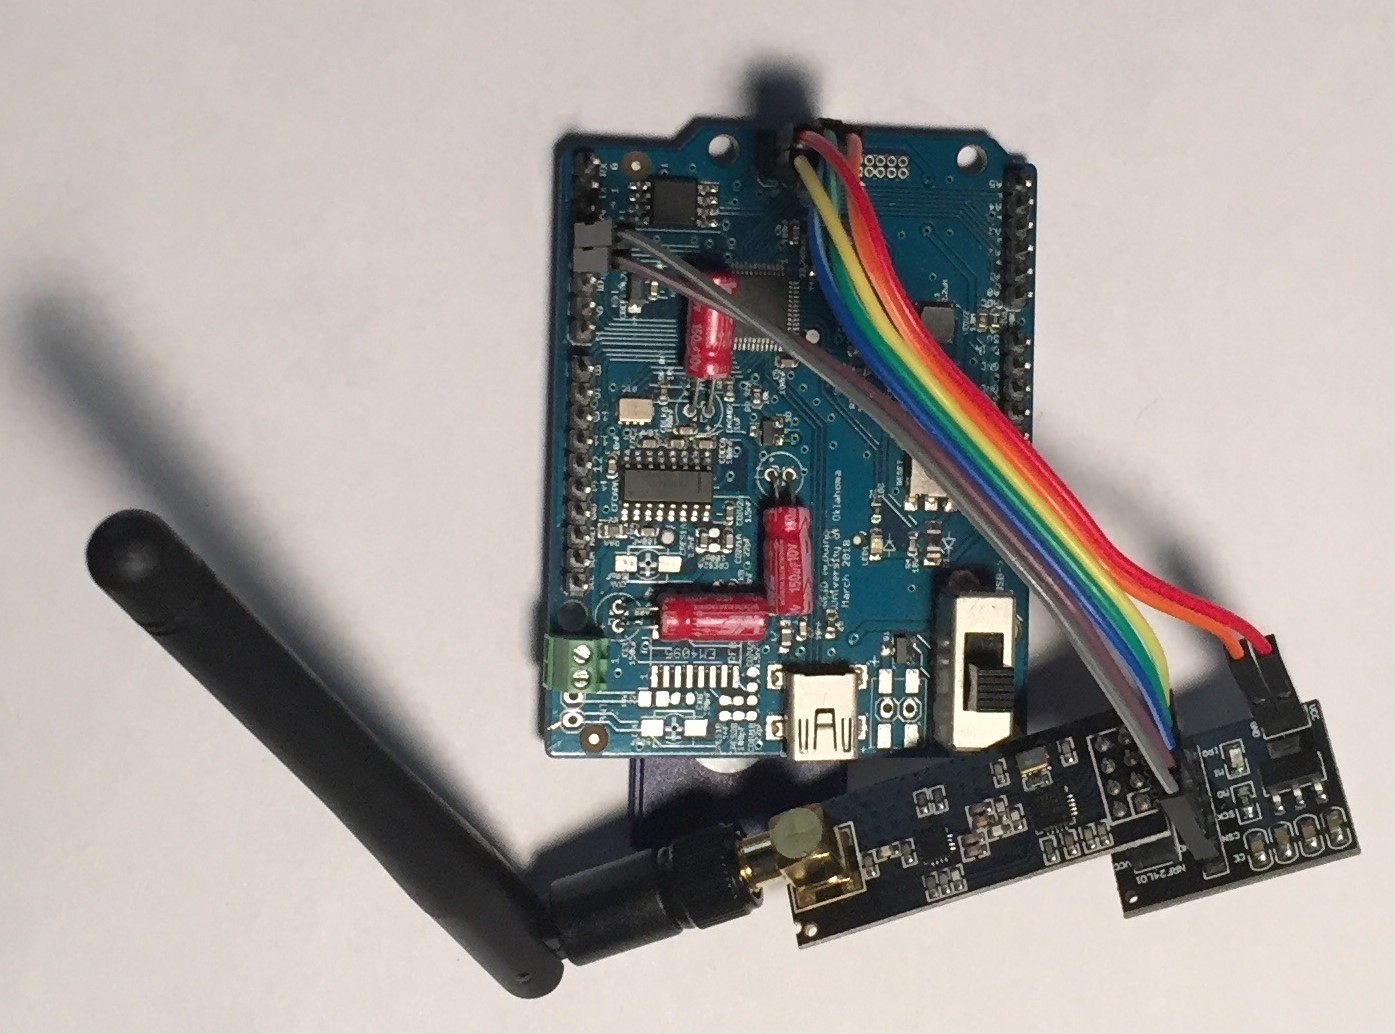
\includegraphics[width=6in,angle=180]{ETAG_Assembled}\\
	ETAG with headers soldered on and female jumper wire connecting long range nRF24 with power module to board (note that CE is connected to 2 and CSN is connected to 3).
\end{center}
This is all that needs to be done to setup the hardware on Arduino based RFID readers like the ETAG.\\\\\\
\underline{\textbf{General way of adding system (e.g. Gen. 2)}}\\\\
For RFID readers that are \textbf{not Arduino based}, like the Gen. 2, there is a lot of work that needs to be done.  The reason for this is that we need to get the RFID data off of the board and into the code, which is written for Arduinos.  This means that you have to purchase an Arduino, any extra equipment to create an interface between the reader and Arduino and add the radio to it.  Any Arduino should do but I recommend the Arduino Nano as it is common, cheap, low power, and easy to use.  Once you do this attach the radio using the instructions above.\\
Next we need a way to get the data off of the RFID reader.  RFID readers typically have a way for people to configure and see what tags the reader is currently reading.  On the Gen. 2 there is a RS-232 serial port where you can attach a cable and connect it to your computer.  When you connect to it you can view the settings and see what reads are coming into the reader.  This provides us with a way to get the data off of the reader into an Arduino.\\
As Arduinos cannot us USB (without a shield), we'll have to add a device that the Arduino understands, a RS232 to TTL with a null modem.  Attach this to the Gen. 2 and try to secure it with screws.  Make sure that you handle the Gen. 2 with care now as there is a large lever arm attached to the RS232 connector.  Notice that there are 2 rows of 4 pins on the connector.  Attach a wire to ground, VCC and txt pins (you may have to experiment with using the rxt pin).  Check to see if the connector uses 3.3V or 5V (mine used 5V).  Connect that wire to the pin giving that voltage on the reader.  If the voltage of the connector and radio are the same and you only have one pin of that voltage you can plug the VCC cable from the radio into the extra VCC pin on the converter.  Next connect the wire that leads to ground and the last wire to digital pin 5.  This is the setup I went through with my RS232 to TTL converter (link in Appendix).\\
Lastly the Arduino needs to get powered.  If the RFID reader has pins to output power (VCC) then you can solder wires to it and a ground pin.  Make sure that the output voltage on the RFID reader is not greater than the input voltage the Arduino can take.  If that condition holds then connect the VCC wire to the VIN pin on the Arduino and ground wire to the ground pin on the Arduino.  If this is not an option on your RFID reader then you might be able to add wires to the battery powering the reader or just use a separate battery to power the Arduino.\\
\begin{center}
	\colorbox{pink}{gen. 2 setup}
	%\includegraphics[width=6in]{Gen2_Assembled}\\
	Gen. 2 board with RS-232 to TTL and null modem and long range nRF24 connected to Arduino, powered by the Gen.2.
\end{center}

\subsubsection{Software}
If you don't already have the Arduino IDE downloaded it from their \href{https://www.arduino.cc/en/Main/Software}{website} and install it.  The Arduino scripts that work with this system are found in the arduino folder of the repository.  If you haven't already downloaded the \href{http://github.com/BenSDuggan/RFID-Network}{GitHub repository} you should do so now.\\
There are several codes that you can choose to upload.  If you just want to test the code you should upload the send on interval code found in the sendOnInterval folder.  There is a version of the code that works with all boards (sendOnIntervalAll) and one written just for the ETAG (sendOnIntervalETAG) that uses the SD card and RTC on the reader.  If you are using the Gen. 2 or ETAG there is code provided that will read reads off of the antenna with out affecting reader performance.  The Gen. 2 script is called RFIDNetworkGen2 and the ETAG script is called RFIDNetworkeETAG.\\
Once you have selected the code you wish to use, connect the Arduino to the computer using the a USB, check to see that the correct board and port are selected.  You're can now upload the code by clicking the upload button.\\

\subsection{Server}
The server is central brains of the system.  It is responsible for communicating with the RFID readers, saving data, making it viewable and more.  Each field site needs one server.  The server is designed to be a Raspberry Pi (RPi) mini computer.  These are less than \$20 and provide a full Linux interface.  It is recommended to use the Raspberry Pi Zero W as it is small, low power, inexpensive and has WiFi included but it should work with any Raspberry Pi (seen below).

\subsubsection{Hardware}
Which ever RPi you decide to use, it is recommended to use a SD card with at least 16GB of space.  Your RPi might come without the pins soldered on.  If this is the case then solder the pins to the board.  Pin 1 is the closest to the middle and the SD slot and pin 2 is next to in on the other long set of pins.  You can view the Raspberry Pi pins at \href{https://pinout.xyz/}{pinout.xyz/}.\\
In addition to the RPi you will need a radio for it and a real time clock (RTC).  The RTC allows the RPi to know what time it is, which is not possible in the field where there is no internet.  The RTC module connects to the RPi using pins 1,3,5,7,9 with pin 1 connected to the VCC (+) pin on the RTC.  Next the radio needs to be connected per the table below.
\begin{center}
	Table showing pin connections between radio and Rapsberry Pi.
	\begin{tabularx}{\textwidth}{ |X|X||X|X| }
		\hline
		\multicolumn{2}{|c||}{\textbf{Power module (from module)}} & \multicolumn{2}{|c|}{\textbf{Capacitor (from radio)}}\\
		\hline
		\textbf{nRF24 pins} & \textbf{RPi pins} & \textbf{nRF2 ins} & \textbf{RPi pins}\\ 
		\hline
		1. GND & Pin 20 & 1. GND & Pin 20 \\ 
		\hline
		2. VCC & Pin 4 & 2. VCC & Pin 17 \\ 
		\hline
		3. CE & Pin 22(GPIO 25) & 3. CE & Pin 22(GPIO 25) \\ 
		\hline
		4. CSN & Pin 24 & 4. CSN & Pin 24 \\ 
		\hline
		5. SCK & Pin 23(GPIO 11) & 5. SCK & Pin 23(GPIO 11) \\ 
		\hline
		6. MOSI & Pin 19(GPIO 10) & 6. MOSI & Pin 19(GPIO 10) \\ 
		\hline
		7. MISO & Pin 21(GPIO 9) & 7. MISO & Pin 21(GPIO 9) \\ 
		\hline
		8. IRQ & not used & 8. IRQ & not used \\ 
		\hline
	\end{tabularx}
\end{center}
The RPi should now look like this:
\begin{center}
	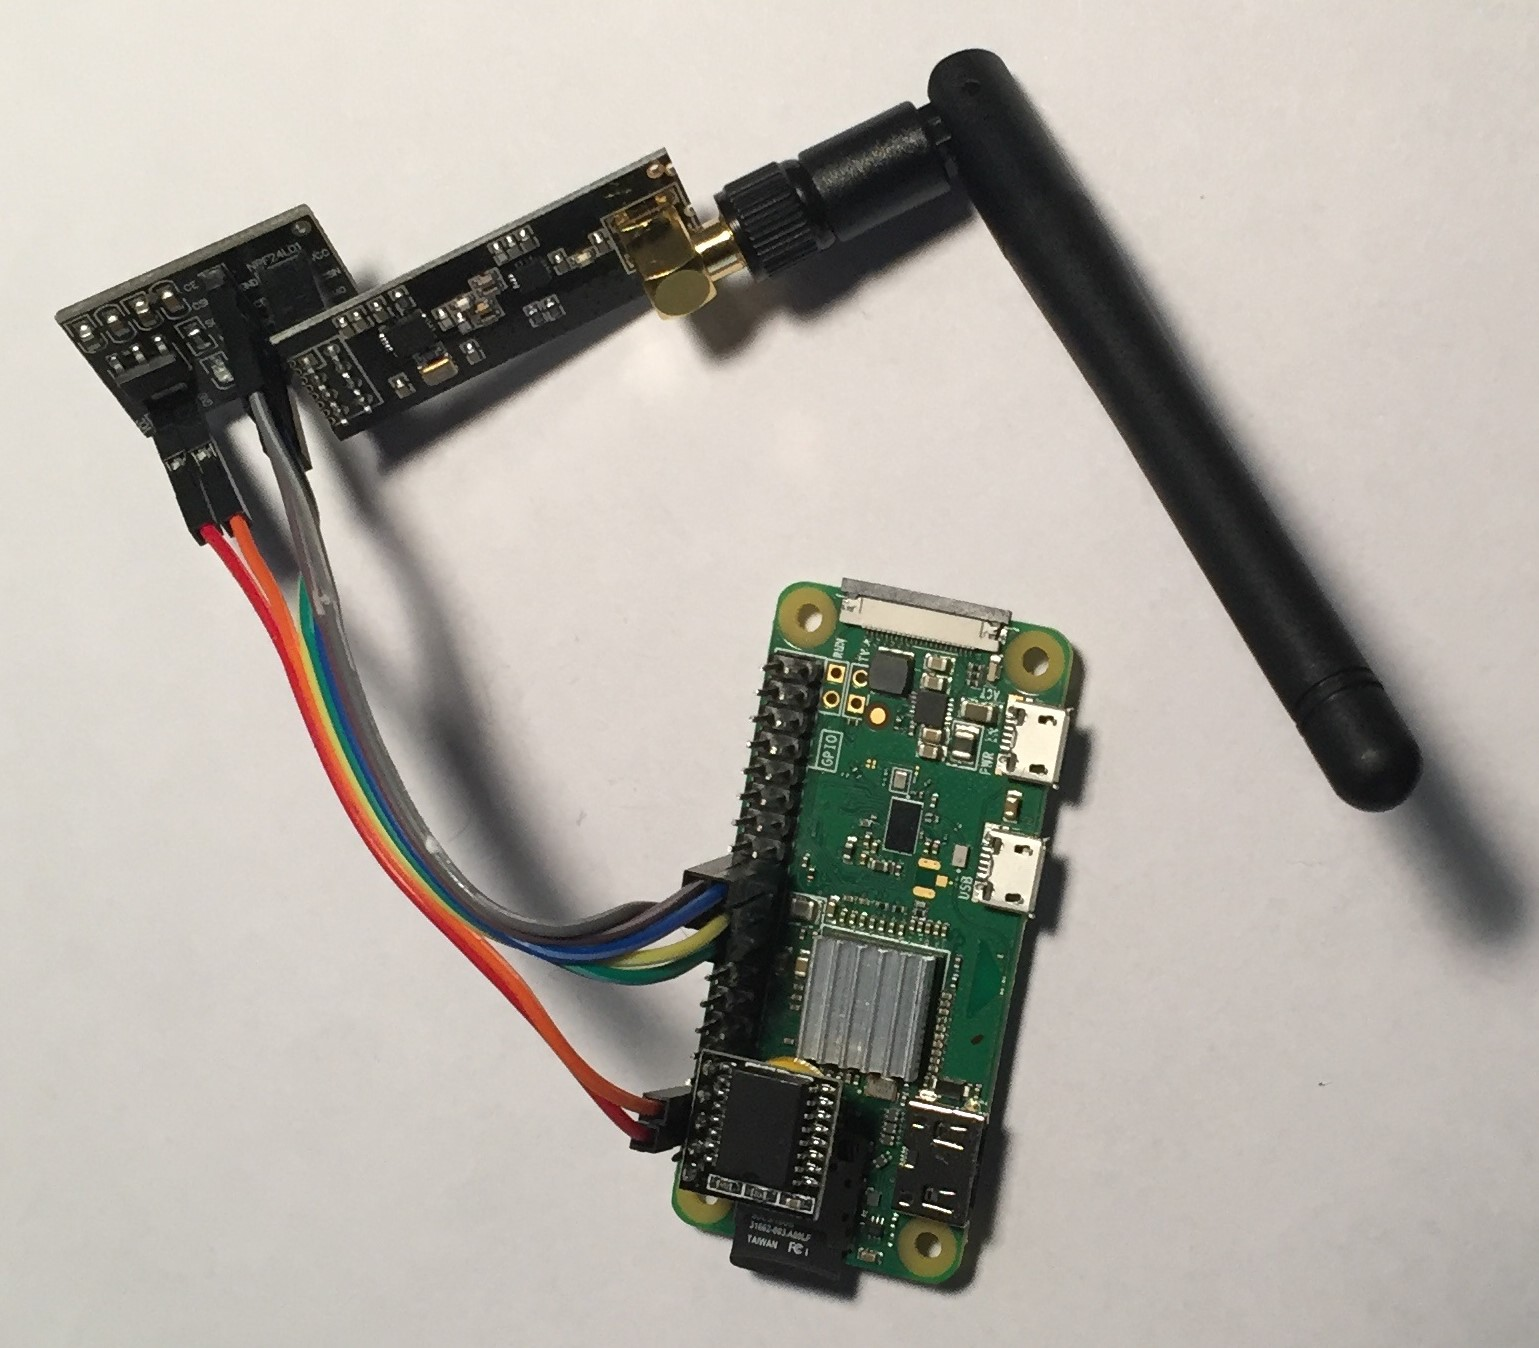
\includegraphics[width=6in]{RPi_Assembled}\\
	Raspberry Pi Zero W with RTC and radio.
\end{center}

\subsubsection{Software}
Download the zip of the NOOBs (new out of box) operating system for the Raspberry Pi found at \url{https://www.raspberrypi.org/downloads/noobs/}.  Unzip the folder and install it according the the readme instructions to setup the SD card.  This is different depending on your operating system but you need to format the SD card and then copy the extracted contents of the NOOB zip onto them.  Next you can plug the SD card into the RPi, add the RTC and radio, plug in a monitor and keyboard and then plug the power cord in.  \textbf{Make sure that you plug the power cable into the correct port (there are two that look the same on the Raspberry Pi zero W).}  Follow the steps on screen to install the operating system.  Make sure that you set the timezone, change the password, connect to WiFi and update the system.  If you have problems with this step you can refer to this video \url{https://www.youtube.com/watch?v=iJbjAJpJA84}.\\
Now you need to install the RFID Network software.  This can be done automatically or manually.  The manual installation instructions, which are incredibly tedious, are found in the following path: RFIDNetwork\_RPi\_install\_list.md.  For that reason you probably want to use the automatic script.  Start by opening the terminal by clicking the icon in the top left corner that is a gray rectangle with white text that looks like "$>$\_" (shown below).  If you only have a key board plugged in you can click the windows key, arrow down to Accessories, arrow right, arrow down to Terminal and press enter.\\
\begin{center}
	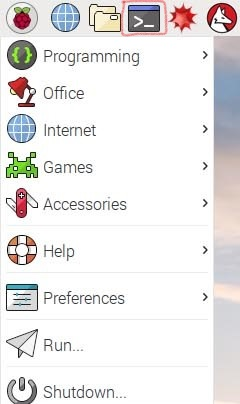
\includegraphics[height=3in]{RPi_desktop}\\
	RPi desktop showing terminal icon.
\end{center}
The terminal is a text only interface where you type commands and then run them by typing enter.  Type "wget https://bit.ly/2CCI6Ok" then press enter.  Next type "chmod +x 2CCI6Ok" and press enter.  Finally type "./2CCI6Ok" and type enter.  This will start the instillation process.  It's recommended that you type "y" when promoted to enter a yes or no answer.  You will be prompted to enter the current password for the Raspberry Pi.  This is needed to configure the database.  You will then be asked to enter an admin username and password.  This is used as the credentials for the database so you should remember it and make it secure.  After the instillation is complete, press y to reboot.  Next you can connect to the access point created by the RPi using a computer or phone.  When prompted to enter a username enter `admin` and password enter `pass`.  Then click on the settings page->Go to Admin Settings and change the admin and username password (still needs to be implemented, will be in 0.9.1).


\section{Server (Raspberry Pi)}
\subsection{How to use}

\subsection{Settings}

\subsection{Battery management system}
The website has a simple way to keep track of the remaining life of the battery.  As the system doesn't have access to the actually remaining battery life it is estimated using the the average power consumption of the board, battery capacity and the date when the battery was changed last.  The data for this is stored in the boxes table of the database with the name `\colorbox{pink}{mysql table name; standardize across boxes.html and database}'.  If you won't wish to use the feature then simply ignore it and nothing will be effected.\\

This feature works by calculating the estimated time the reader can stay on using the calculation below:
\begin{center}
	reader on time $= \frac{battery capacity (mAH)}{average power consumption} $
\end{center}
The battery capacity is a figure found on the battery you're using while the average power consumption can be calculated theoretically or found experimentally.  To calculate the theoretical average power consumption you can use the formula below:
\begin{center}
	average power consumption $= \frac{t_{awake} \cdot \frac{t_{pollTime} \cdot I_{antennaCurrent} + t_{pauseTime} \cdot I_{idleCurrent}}{t_{poll time} + t_{sleep}} + t_{sleep} \cdot I_{sleep}}{t_{awake} + t_{sleep}}  $
\end{center}
The table below shows what each variable means and the approximate values for those variables on the ETAG and Gen. 2 board:
\begin{center}
	\begin{tabularx}{\textwidth}{ |X|c|X|X| }
		\hline
		\textbf{Variable} & \textbf{Meaning} & \textbf{ETAG value} & \textbf{Gen.2 value} \\ 
		\hline
		$t_{awake}$ & hours board spends on during 1 day & 14 H & 14 H \\ 
		\hline
		$t_{pollTime}$ & milliseconds antenna spends on during poll & 300 ms & 300 ms \\ 
		\hline
		$I_{antennaCurrent}$ & milliamps the board uses while scanning for tags & 125 mA & 45 mA \\ 
		\hline
		$t_{pauseTime}$ & milliseconds antenna spends on during poll & 100 ms & 100 ms \\ 
		\hline
		$I_{idleCurrent}$ & milliamps the board uses while on but not scanning  & 11 mA & \colorbox{pink}{need number} mA \\ 
		\hline
		$t_{sleep}$ & hours board spends on during 1 day & 10 H & 10 H \\ 
		\hline
		$I_{sleep}$ & milliamps the board uses while sleeping  & 1 mA & \colorbox{pink}{need number} mA \\ 
		\hline
	\end{tabularx}
	*Note: $t_{sleep} + t_{awake}$ should equal 24 hours
\end{center}
This method gives a rough estimate of the average power consumption but it not alway easy for people to calculate this number.  A simpler way to find the average power consumption is to determine how long the reader stays on a given set of parameters.  Then you can calculate the average power consumption using the following formula:
\begin{center}
	 average power consumption mA = $ \frac{battery\:capacity(mA \cdot H)}{on\:time(H)}$\\
	 *Note: The average power consumption will change if any of the RFID reader settings change
\end{center}
Once the estimated time the board can stay on has been calculated it is compared with the last time the battery was changed.  The time remaining and percent time remaining on is calculated using the formulas below:
\begin{center}
	time remaining on = reader on time - [current time since epoch (hours) - battery change time since epoch (hours)]\\
	percent time remaining = $\frac{time\:remaining\:on}{reader\:on\:time} \cdot 100\%$
\end{center}
The battery change time for a reader can be changed to the current time by clicking the on the reader and then clicking the ``Change battery button''.  The date can be manually set by clicking on the reader, clicking edit and then changing the date-time.\\

The results for these calculations are shown in two ways: if you look at a reader then you can see the estimated date that the reader will die or you can look at the color of the row.  The row color represents the percent battery life remaining and the colors have the following values:

\subsection{Front-end (website)}
This section is intended to help people understand how the front-end web code is written.  This section should help with adding new pages or editing existing ones.\\  
The web front-end is designed using HTML, CSS and JavaScript and relies heavily on Socket.io (seamless communication between client and sever via web sockets), jQuery (better JavaScript) and Bootstrap (cohesive design).

\subsubsection{Style}
The styling is done using Bootstrap v4.0.0-beta.3.  The style and script files are loaded in the header section of each page.  For a consistent theme use the bootstrap classes outlined below.  You can see an example page in "template.html" and use it to make custom pages.  Additionally the \href{https://getbootstrap.com/docs/4.2/getting-started/introduction/}{Bootstrap documentation} should help with most of your formating concerns.\\

\begin{lstlisting}[language=html, caption="template.html", breaklines=true]
<!--
* Ben Duggan
* 8/8/18
* Basic page framework
-->

<!DOCTYPE html>
<html>
<head>
	<meta charset="utf-8">
	<meta name="viewport" content="width=device-width, initial-scale=1, shrink-to-fit=no">
	
	<title>Template - RFID Network</title>
	
	<link href="/dependences/bootstrap/css/bootstrap.min.css" rel="stylesheet">
	<link href="/dependences/main.css" rel="stylesheet">

	<script src="/dependences/jsLibraries/jquery-3.2.1.min.js"></script>
	<script src="/dependences/bootstrap/js/bootstrap.min.js"></script>
	<script src="/socket.io/socket.io.js"></script>
	<script src="/dependences/main.js"></script>
</head>
<body>
	<nav class="navbar navbar-expand-md navbar-dark bg-primary">
		<a class="navbar-brand" href="/">RFID Network</a>
		<button class="navbar-toggler" type="button" data-toggle="collapse" data-target="#navbarNavDropdown" aria-controls="navbarNavDropdown" aria-expanded="false" aria-label="Toggle navigation">
		<span class="navbar-toggler-icon"></span>
		</button>
		<div id="navbarNavDropdown" class="navbar-collapse collapse">
			<ul class="navbar-nav mr-auto">
				<li class="nav-item active"><a class="nav-link" href="/birds.html">Birds</a></li>
				<li class="nav-item"><a class="nav-link" href="/readers.html">Reader</a></li>
				<li class="nav-item"><a class="nav-link" href="/settings.html">Settings</a></li>
				<li class="nav-item"><a class="nav-link" href="/logs.html">Logs</a></li>
				<li class="nav-item"><a class="nav-link" href="/help.html">Help</a></li>
			</ul>
		</div>
	</nav>
	<div id="errorsContainer"></div>
	<div class="container container-main">
	</div>
</body>
</html>
\end{lstlisting}


\underline{\textbf{Navigation bar}}\\\\
The navigation bar should be the first item placed at the top of each page.  This is the default navigation bar.  If you want to add a tab to a page you simply need to copy the list item (li), change the href and display text.  Copy this across each html document.  The class "active" should be added to the list item who's href matches the html page you're on (so this code came from birds.html as the active class is one of it's attributes).\\  The navigation bar automatically compacts on mobile screens and replaces the tabs with a hamburger (3 lined bar) which can be clicked to display the pages.

\begin{lstlisting}[language=html, caption="Navigation bar style", breaklines=true]
<nav class="navbar navbar-expand-md navbar-dark bg-primary">
	<a class="navbar-brand" href="/">RFID Network</a>
	<button class="navbar-toggler" type="button" data-toggle="collapse" data-target="#navbarNavDropdown" aria-controls="navbarNavDropdown" aria-expanded="false" aria-label="Toggle navigation">
	<span class="navbar-toggler-icon"></span>
	</button>
	<div id="navbarNavDropdown" class="navbar-collapse collapse">
		<ul class="navbar-nav mr-auto">
			<li class="nav-item active"><a class="nav-link" href="/birds.html">Birds</a></li>
			<li class="nav-item"><a class="nav-link" href="/readers.html">Reader</a></li>
			<li class="nav-item"><a class="nav-link" href="/settings.html">Settings</a></li>
			<li class="nav-item"><a class="nav-link" href="/logs.html">Logs</a></li>
			<li class="nav-item"><a class="nav-link" href="/help.html">Help</a></li>
		</ul>
	</div>
</nav>
\end{lstlisting}


\underline{\textbf{Error bar and main div}}\\\\
After the navigation bar you should add a div where errors can be placed with id=errorsContainer.  The back-end will attempt to send an error to all users whenever one is detected so it is good to add this feater to each page.  After the error div you should add a div with classes "container" and "container-main".  All the code that is normally displayed, apart from the nav bar and any scripts loaded after the body, should be placed in this main div.  This ensures that the proper margins and padding will be kept across the page.

\begin{lstlisting}[language=html, caption="Error bar and main div", breaklines=true]
<div id="errorsContainer"></div>
<div class="container container-main">
	<!-- Place your html code here -->
</div>
\end{lstlisting}

\underline{\textbf{Other styling items}}\\\\
When placing items next to each other it is best to use a grid.  This allows the content to be dynamically resized when the screen size reaches a certain resolution.  
\begin{lstlisting}[language=html, caption="Bootstrap grid", breaklines=true]
<div class="row">
	<div class="col-md-4">
		<!-- cell 1 -->
	</div>
	<div class="col-md-4">
		<!-- cell 2 -->
	</div>
	<div class="col-md-4">
		<!-- cell 3 -->
	</div>
</div>
\end{lstlisting}

Tables are used to display lots of data.  All tables use the stripped class, except when adding coloring (like with the battery management).
\begin{lstlisting}[language=html, caption="Bootstrap table", breaklines=true]
<table class="table table-striped">
	<thead>
		<tr>
			<th>Header 1</th><th>Header 2</th>
		</tr>
	</thead>
	<tbody>
		<tr>
			<td>Body 1</td><td>Body 2</td>
		</tr>
	</tbody>
</table>
\end{lstlisting}

Most buttons use the primary class as it goes with the overall blue color scheme.
\begin{lstlisting}[language=html, caption="Bootstrap button", breaklines=true]
<button type="button" class="btn btn-primary" id="button-id">Button text</button>
\end{lstlisting}

\subsubsection{Scripting}
The scripting on the front-end is done using JavaScript with jQuery (better js), socket.io (server-client communication), select2(auto complete inputs) and chart.js (creates nice looking charts).  Not every page needs to include select2 and chart.js but you should include jQuery and the main.js script found in the dependencies folder.  


\underline{\textbf{main.js}}\\\\
The main.js script, found in RFID-Network/server/dependencies/main.js, is used to setup several variables, methods and page settings.  The most important thing this script does is create a socket.io instance named \textit{socket}.  \textit{socket} can be used in any other script called after main.js.  Look at the \href{https://socket.io/docs/client-api/}{socket.io client documentation} to see how to use the library.  The script also adds a prototype method called \textit{toSQLString} to the Javascript Date class.  This method is used to convert a Javascript Date object to the correct MySQL format (also great for human readability).  There are methods that check to see if the connection to the server is lost or gained.  Finally, \textit{socket.on("errorMessage")} that displays errors at the top of the screen when one happens.

\begin{lstlisting}[language=html, caption="main.js", breaklines=true]
/*
* Ben Duggan
* 12/14/18
* Reusable javascript code used by most pages
*/

var socket = io();
var wasDisconnected = false;

// Fixes the problem of ISO style with timezone offset
// Solution from - https://stackoverflow.com/questions/17415579/how-to-iso-8601-format-a-date-with-timezone-offset-in-javascript
Date.prototype.toSQLString = function() {
	var tzo = -this.getTimezoneOffset(),
		dif = tzo >= 0 ? '+' : '-',
		pad = function(num) {
		var norm = Math.floor(Math.abs(num));
		return (norm < 10 ? '0' : '') + norm;
		};
	return this.getFullYear() +
		'-' + pad(this.getMonth() + 1) +
		'-' + pad(this.getDate()) +
		' ' + pad(this.getHours()) +
		':' + pad(this.getMinutes()) +
		':' + pad(this.getSeconds());
}

socket.on('connect', function(data) {
	if(wasDisconnected) {
		$('#error-connection').remove();
		$('#errorsContainer').prepend('<div class="alert alert-success alert-dismissible fade show" id="error-connection" role="alert"><strong>Connected to the server. </strong><button type="button" class="close" data-dismiss="alert" aria-label="Close"><span aria-hidden="true">&times;</span></button></div>');
		wasDisconnected = false;
	}
});

socket.on('disconnect', function(data) {
	console.log(data);
	$('#error-connection').remove();
	$('#errorsContainer').prepend('<div class="alert alert-danger alert-dismissible fade show" id="error-connection" role="alert"><strong>Disconnected from the server. </strong>The server might have crashed.  This means that no data is being saved.  Try refreshing and if nothing appears, restart the server.<button type="button" class="close" data-dismiss="alert" aria-label="Close"><span aria-hidden="true">&times;</span></button></div>');
	wasDisconnected = true;
});

socket.on('errorMessage', function(data) {
	console.error(data);
	
	var err = '';
	for(var c in data) {
		err += "{<i>" + c + "</i>: " + data[c] + "} ";
	}
	
	$('#errorsContainer').prepend('<div class="alert alert-danger alert-dismissible fade show" role="alert"><strong>An error occured on the server: </strong>'+err+'<button type="button" class="close" data-dismiss="alert" aria-label="Close"><span aria-hidden="true">&times;</span></button></div>');
});
\end{lstlisting}


\underline{\textbf{Reads Viewer}}\\\\
The reads view displays the reads stored on the server and provides tools for subsetting and viewing the reads.  There are three parts of the viewer.  The first section is a filter that lets you enter tags, a date range or other parameters to filter the data by.  The filtering works by concatenating each filter field into a long SQL string.  This means that if you enter a RIFD tag and a box but that tag was never at the box nothing will show up.  The second section shows bird and box analytics.  The last section shows the raw reads.  To add the reads viewer to a page place a div tag with id \textit{readsViewer} where you want the viewer to be placed.  Then add a script with src "/dependences/readsViewer.js" at the end of the body tag.  To load the content you need to call \textit{rvLoad()}.  You can load a filter by calling \textit{rvSetFilter({})} and placing a JSON object with the desired filter as a parameter (e.g. {rfid:["A0B1C2D3E4"]}).  You can also hide the content by calling \textit{rvHide()}.  You can see an example of how to use this below.

\begin{lstlisting}[language=html, caption="Reads viewer", breaklines=true]
<html>
<head>
	<link href="dependences/bootstrap/css/bootstrap.min.css" rel="stylesheet">
	<link href="dependences/main.css" rel="stylesheet">
	
	<script src="/dependences/jsLibraries/jquery-3.2.1.min.js"></script>
	<script src="dependences/bootstrap/js/bootstrap.min.js"></script>
	<script src="/socket.io/socket.io.js"></script>
	<script src="/dependences/main.js"></script>
</head>
<body>
	<div id="readsViewer"></div>
	<script src="/dependences/readsViewer.js"></script>
	<script>
		$('document').ready(function() {
			rvSetFilter({rfid:["A0B1C2D3E4"]}); // Set filter
			rvLoad(); // Load viewer into div with id "readsViewer"
		});
	</script>
</body>
</html>
\end{lstlisting}


\underline{\textbf{Socket calls}}\\\\
Socket.io is used to make a TCP websocket channel to allow for quick and seamless communication between the server and client.  There are a variety of socket calls which can be made from the website and additional several things the website listens for.  Here is a list of calls that the website can make to the server and the data they send.
\begin{center}
	Website socket.emit calls.
	\begin{tabularx}{\textwidth}{ |X|X|X| }
		\hline
		\textbf{Name} & \textbf{Data} & \textbf{Usage}\\ 
		\hline
		&  & \\ 
		\hline
		
		
		
	\end{tabularx}
\end{center}


\begin{lstlisting}[language=html, caption="aaa", breaklines=true]

\end{lstlisting}

\subsection{Back-end (Node.js)}

\section{RFIDNetwork class (Arduino code)}
\subsection{Documentation}
\subsection{How to add to another reader}
\subsection{Understanding the mesh networking}

\section{Protocols}
\subsection{RFIDNetworkProtocol}

\subsection{Localized radio sleep}
	\subsubsection{Purpose}
	There are two versions of the nRF24 radios commonly available: the short range and long range models.  Based off our testing the short range antennas don't provide sufficient performance as they have a small range, <100 m, and don't poses the capability to transmit through our junction box enclosures.  For this reason the long range antennas must be used.  These antennas consume around 24-26 mA during all power and data rate settings and < 1 mA when they power down, or sleep.  Additionally, the radios aren't always transmitting.  They only transmit when they get a new RFID read or need the time updated.

\section{Tests}
\subsection{Range}
\subsection{Power}
\subsection{Reliability}

\section{Appendix}
\subsection{Purchase list}
Below is the table with the list of items that you to use this system.
\begin{center}
\begin{tabularx}{\textwidth}{ |X|X|X|X|X| }
	\hline
	\textbf{Item} & \textbf{Description} & \textbf{~Price} & \textbf{Link} & \textbf{Usage}\\ 
	\hline
	Long range NRF24L01 + PA + LNA & Radio used by all components in system & \$ 4.50 & \url{http://a.co/d/gTyLiEB} & All \\ 
	\hline
	*nRF24 power module & des & \$2.00 & \url{http://a.co/d/4aO5gxl} & All \\ 
	\hline
	*4.7$\mu$F & capsitor soldered to pin 1\&2 on nRF24 to fix power & \$0.10 & \url{http://a.co/d/geAsuhP} & All \\ 
	\hline
	Female-to-female jumper wires & Connect components in the system & \textless\$0.10 & \url{http://a.co/d/8rEd3eV} & All \\ 
	\hline
	*5V Arduino Nano & Arduino used to interface with Gen. 2 & \$4.50 & \url{http://a.co/d/9YXtAxh} &  Gen. 2 \\ 
	\hline
	*RS-232 to TTL converter & Converts Gen.2 communication to Arduino communication & \$6.49 & \url{http://a.co/d/5TbXOCu} & Gen. 2 \\ 
	\hline
	*Null modem & Lets the converter work with the gen. 2 & \$3.50 & \url{http://a.co/d/6bGmY3q} & Gen. 2 \\ 
	\hline
	Raspberry Pi Zero W & Low power RPi with WiFi & \$20 & \url{http://a.co/d/99oZjQa} & Server \\ 
	\hline
	16Gb micro SD card & SD card for storage on the RPi & \$11.00 & \url{http://a.co/d/f0VfbtY} & server \\ 
	\hline
	DS3231 RTC & RTC used with RPi & \$2.10 & \url{http://a.co/d/elzvuFW} & Server \\ 
	\hline
	item & des & price & \url{} & use \\ 
	\hline
	
\end{tabularx}
*Denotes not required
\end{center}

\subsection{Code documentation/walk through}
\subsection{Dependencies}
This section lists the dependence and versions used when building and testing the system.\\
\begin{center}
	\begin{tabularx}{\textwidth}{ |X|X|X|X| }
		\hline
		\textbf{Dependency} & \textbf{Version} & \textbf{Usage} & \textbf{Link}\\ 
		\hline
		Raspberry Pi Noobs (Raspian) & 3.0.0 & Raspberry Pi OS & \url{https://www.raspberrypi.org/}\\ 
		\hline
		node.js & v9.9.0-linux-armv6l & Creates a Javascript server. & \url{https://nodejs.org/en/}\\ 
		\hline
		 &  &  & \url{}\\ 
		\hline
		 &  &  & \url{}\\ 
		\hline
		 &  &  & \url{}\\ 
		\hline
		 &  &  & \url{}\\ 
		\hline
		Bootstrap & v4.0.0-beta.3 & Web page styling & \url{https://getbootstrap.com/}\\ 
		\hline
		Socket.IO & v2.1.1 & server/client TCP web sockets & \url{https://socket.io/}\\ 
		\hline
		Select2 & 4.0.6-rc.0 & Drop down that auto fills input forms on the website & \url{https://select2.org/}\\ 
		\hline
		Chart.js & v2.7.2 & Creates nice looking, interactive charts on the website & \url{http://chartjs.org/}\\ 
		\hline
		 &  &  & \url{}\\ 
		\hline
		
		
		  
	\end{tabularx}
\end{center}

\end{document}